\documentclass[graphics]{beamer}

\usepackage{graphicx}
\usepackage{verbatim}
\usepackage{wrapfig}
\useoutertheme{shadow}
%\usecolortheme{orchid}
\usecolortheme{seahorse}


% math commands
\newcommand{\be}{\begin{eqnarray}}
\newcommand{\ee}{\end{eqnarray}}
\newcommand{\beq}{\begin{equation}}
\newcommand{\eeq}{\end{equation}}
\def\simless{\mathbin{\lower 3pt\hbox
      {$\rlap{\raise 5pt\hbox{$\char'074$}}\mathchar"7218$}}}
\def\simgreat{\mathbin{\lower 3pt\hbox
      {$\rlap{\raise 5pt\hbox{$\char'076$}}\mathchar"7218$}}} %> or of order

% variables

\def\toonscale{0.45}
\def\mboxy#1{\mbox{\small #1}}


\begin{comment}
\AtBeginSection[]{
  \frame{
    \frametitle{Outline}
    \tableofcontents[currentsection]
  }
}
\end{comment}

\title{Pulsar Lensing
}
\subtitle{}
\author[U. Pen]{Ue-Li Pen, M. van Kerkwijk, K. Vanderlinde and many more
\\[8mm] 
}
\date{Oct 7, 2015}


\begin{document}

\frame{
%\vspace{-2.3in}
%\begin{center}\hspace{-0.75in} 
%\includegraphics[width=5.4in]{Figures/traverse-aurora.jpg}
%\end{center}
%\vspace{-0.2in}image credit: Andre Recnik
%\vspace{-3in}
\begin{picture}(320,250)
\put(-50,20){
\includegraphics[width=5.5in]{Figures/traverse-aurora.jpg}}
%\textcolor{red}{
image credit: Andre Recnik
\end{picture}
}

%\section*{Introduction}
\section{Pulsar Lensing}

\begin{comment}
  \subsection{Outline}

  \frame{
    \frametitle{Outline}
    \tableofcontents
  }
\end{comment}

  \frame{
\vspace{-0.5in}
    \frametitle{Pulsar VLBI}
    \begin{itemize}
        \item coherent, unresolved point sources
        \item radar/holography imaging through ISM
        \item potential for imaging pulsar magnetosphere, ISM.
%          \vspace{-0.15in}
    \end{itemize}
\vspace{-0.1in}\hspace{.3in}
\includegraphics[width=1.2in]{Figures/DRAO_26m_dish.jpg}
\vspace{-0.5in}
\includegraphics[width=1.9in]{Figures/IMG-7749-ARO-crop.JPG}
  }
  \frame{
    \frametitle{New Pulsar Science}
    \begin{itemize}
        \item use interstellar plasma as telescope
        \item unprecedented angular precision: 50 picoarcseconds
    \end{itemize}
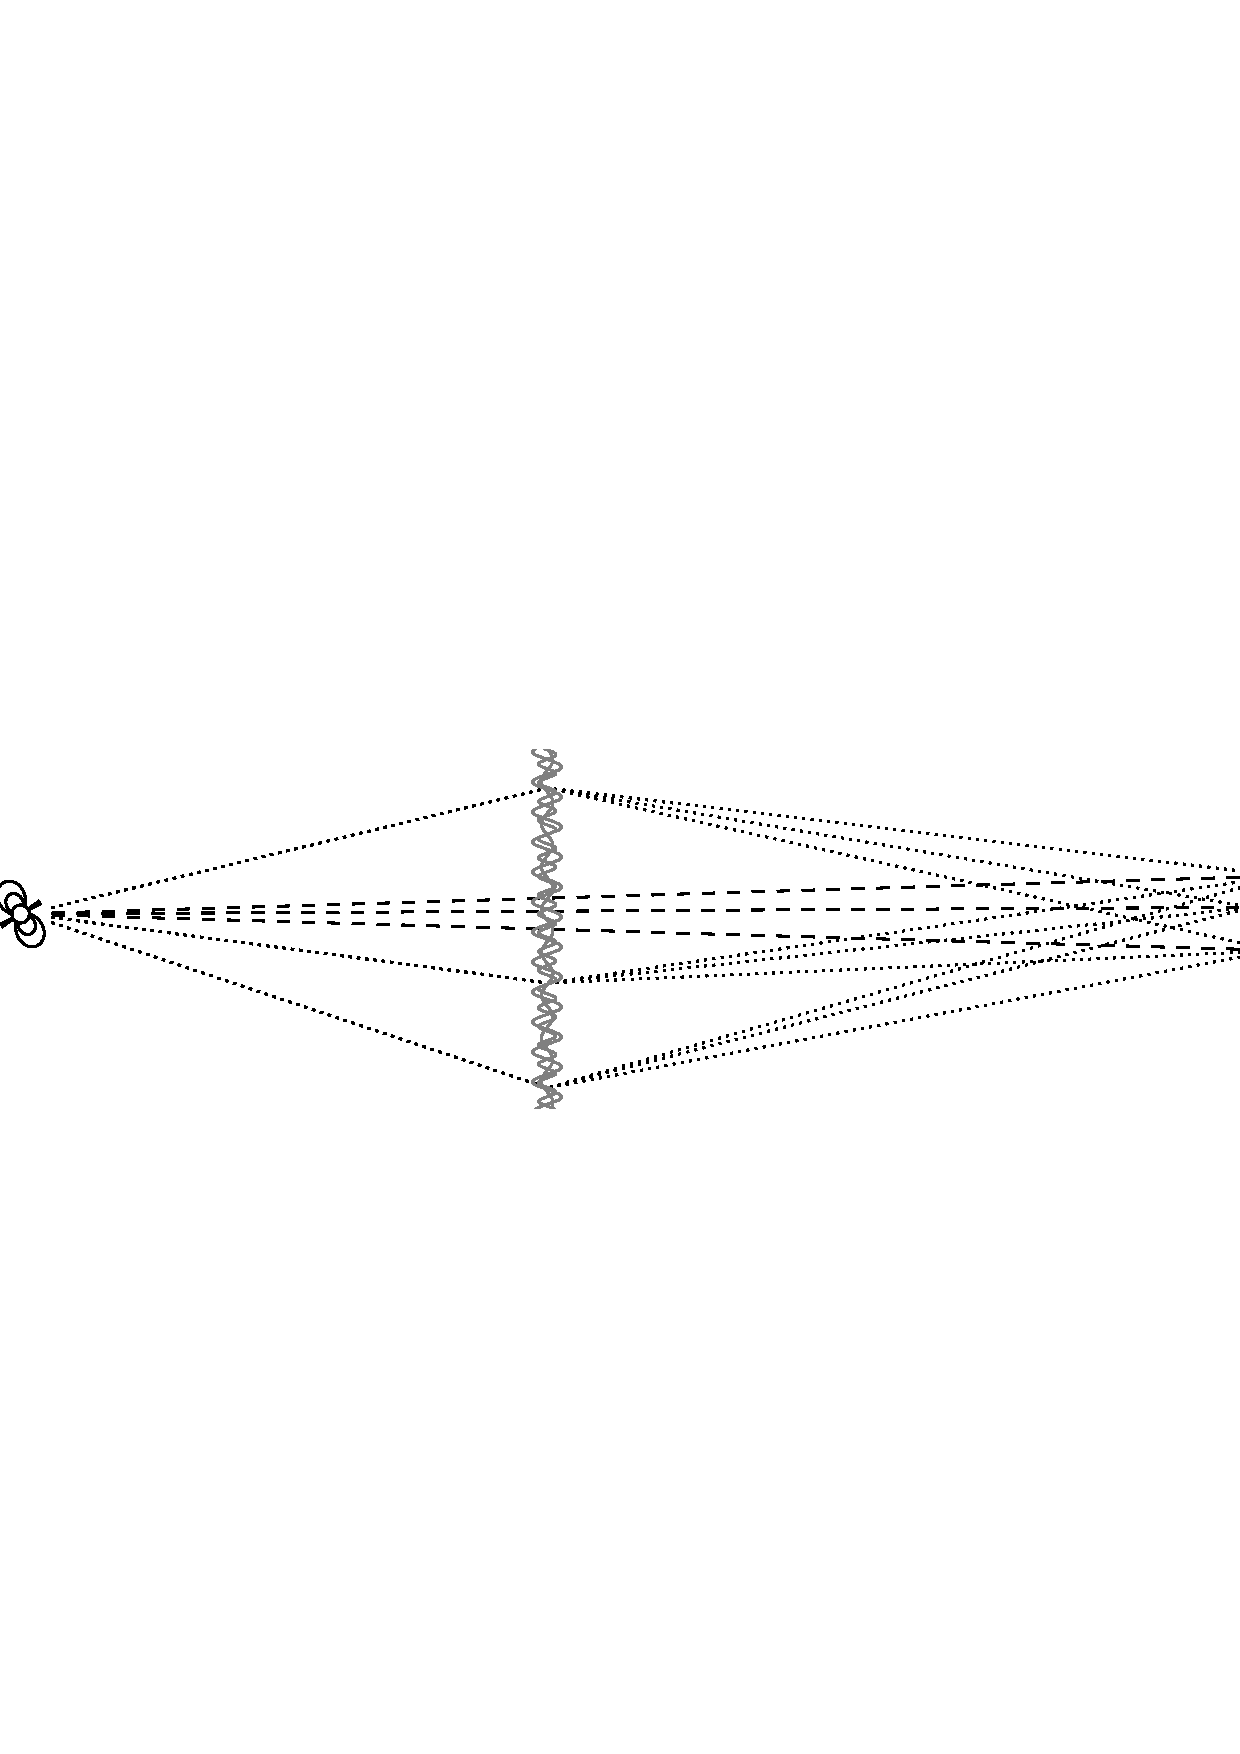
\includegraphics[width=4.5in]{Figures/scintillometry.png}
}

\end{document}
